\section{Epipolar Geometry and Chaining}
\label{egc}
In this section we are going to describe the first step of the Structure from Motion algorithm, which is to exploit prior knowledge about the scene. This is done by finding corresponding image points in multiple views and compute their epipolar geometry which is expressed algebraically by the fundamental matrix which can be decomposed to obtain the required projection matrices.

\subsection{DataSet}
The data we were required to use consisted of two individual datasets. The first one contains 49 frames, each one of them depicting a house from a different view. The second contains 16 frames, each one of them depicting a teddy-bear from a different view. In each frame the camera movement is small, making the process of extracting structure from the scene an easier task.

\subsection{Implementation}
An important step of the algorithm is to identify local features in each image which are consistent in most of the frames. For this purpose we used a Scale-invariant feature transform (or SIFT) (vl\_ sift command from vlFeat library) algorithm to detect points of interest in each frame. In order to restrict the search process of the SIFT detector an active contour based segmentation was used. By applying this technique we were able to segment the frames into background and foreground regions, allowing us to keep only the points that exist on the object of interest as can be seen in figure~\ref{fig:houseBackground}.

\begin{figure}[ht!]
  \centering
    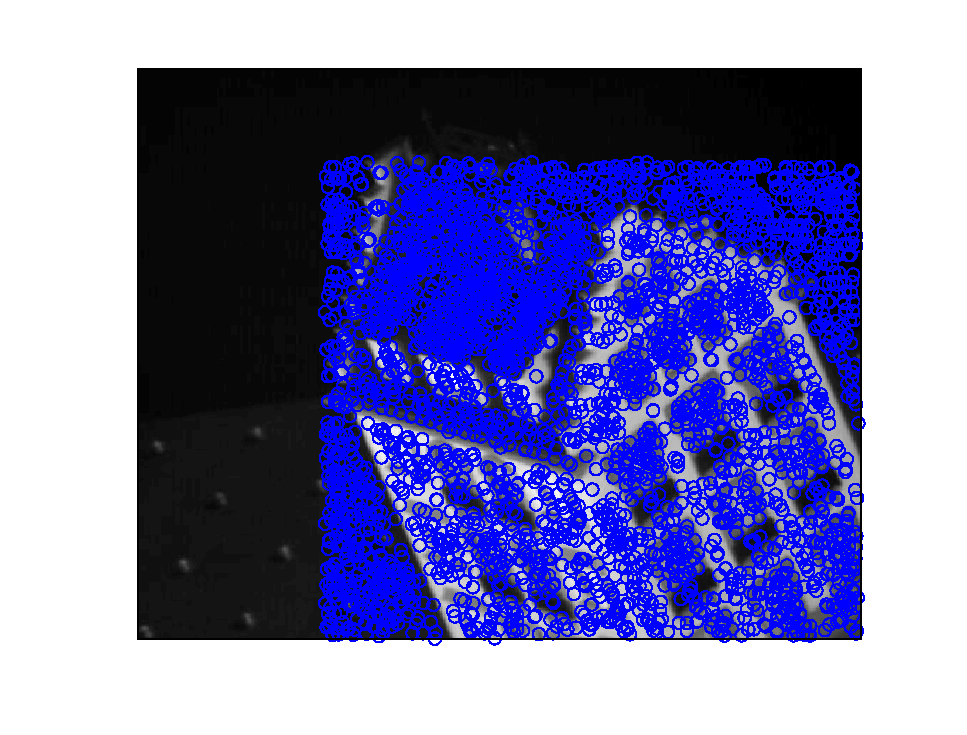
\includegraphics[width=0.49\textwidth]{figures/houseBackground.eps}
    \caption{Feature points extracted by the SIFT detector found on the object of interest}
    \label{fig:houseBackground}
\end{figure}

By finding feature points in every frame we are able to identify matches in each consecutive frame. This is done by using the build-in function vl\_ ucbmatch of the vlFeat library of matlab which returns the qualitative corresponding feature points and rejects the ambiguous ones. The vl\_ sift command without parameter tuning gives only a limited number of feature points as illustrated on the first image of figure~\ref{fig:matches}. By setting a higher edge threshold which is the threshold to filter out edge-like features we were able to obtain more key points. Another parameter we tuned was the number of levels per octave. By increasing this number in principle it returns more refined keypoints, but in practice the selection may be unstable due to noise. Feature matches between two consecutive frames of the House dataset with tuned parameters, is displayed on the second image of figure~\ref{fig:matches}.

\begin{figure}[ht!]
  \centering
    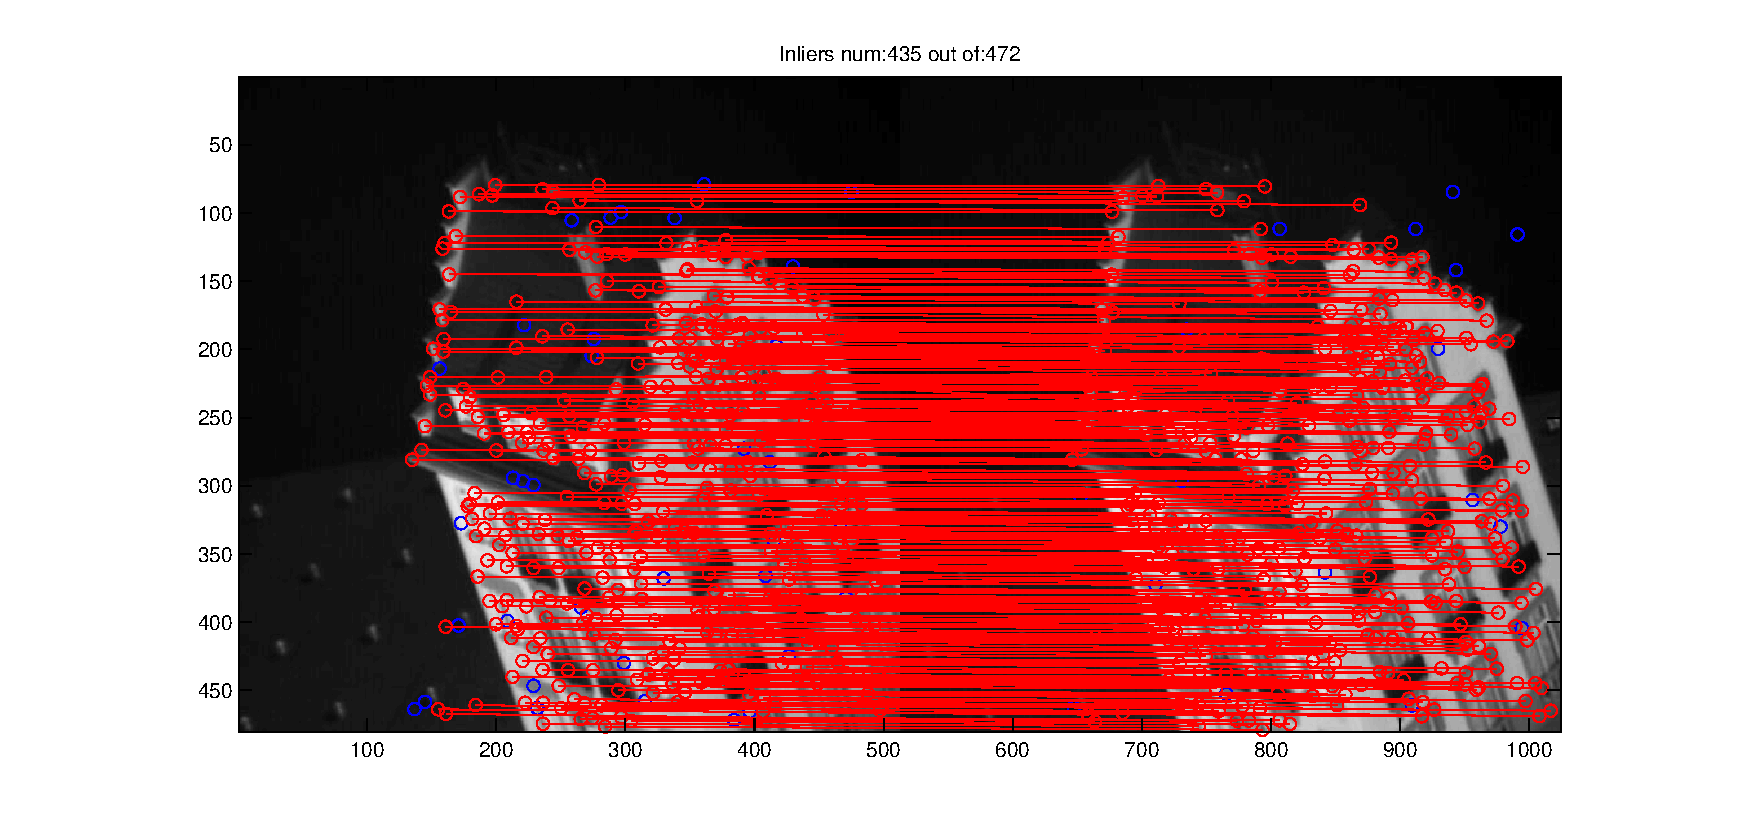
\includegraphics[width=0.55\textwidth]{figures/matchesSimple.eps}\\
    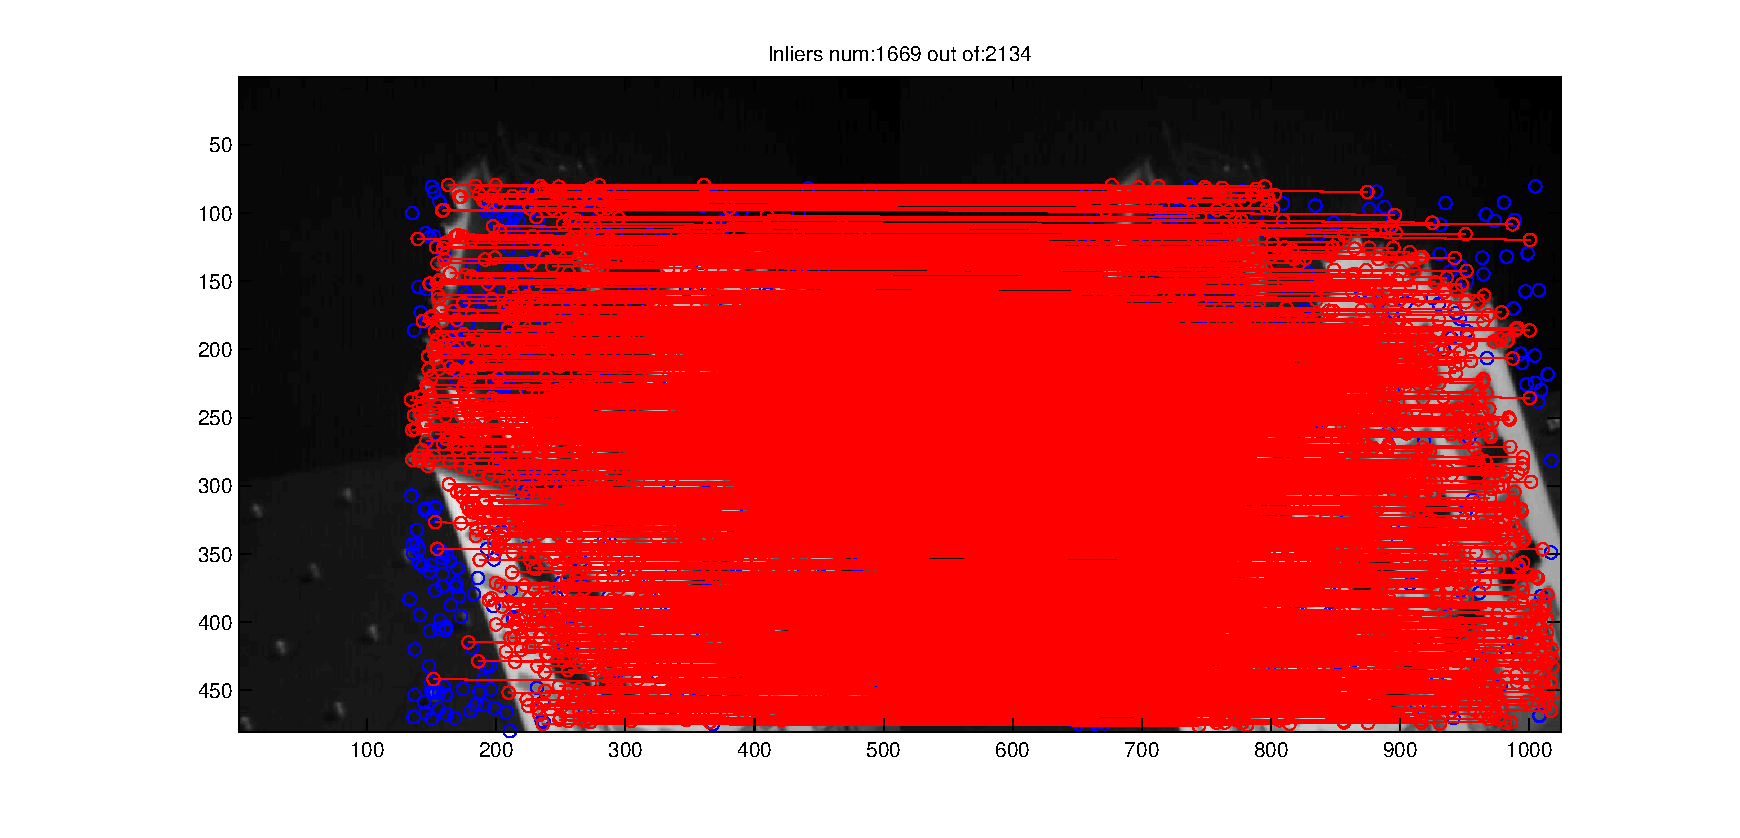
\includegraphics[width=0.55\textwidth]{figures/matchesWithThresh.eps}
    \caption{Above: Feature matches between two consecutive frames without tuned parameters, Below: Feature matches between two consecutive frames with parameter tuning: edgeThresh:30, Levels: 30.}
    \label{fig:matches}
\end{figure}

The next step is to apply centering to the points, namely subtract the centroid of the feature points (remove translation) according to :

\begin{equation}
\hat{x} = x_{ij} - \frac{1}{n} \sum_{k=1}^{n} x_{ik}
\end{equation}

To estimate the fundamental matrix from the corresponding image points extracted by the SIFT detector the normalized ransac eight-point algorithm~\cite{eight-point} was implemented. This variational algorithm leads to a more stable result than the simple eight-point implementation. The steps of the algorithm are:

\begin{enumerate}[1]
  \item Pick 8 random matches from the list of the corresponding points.
  \item Construct a matrix A from the matches and get the transformation matrix from the last column of V of the Singular Value Decomposition of A.
  \item Count the number of inliers (points that agree with the transformation matrix) by computing the Sampson distance (if distance is smaller than a certain threshold then we consider the point as an inlier)
  \item Repeat steps 1 to 3 until the majority of the points are inliers.
\end{enumerate}


\subsection{Chaining}
The last step is to construct the Point View Matrix which contains normalized point coordinates (inliers) which are consistent in all frames. Actually it is not always the case that many points are present in all frames due to the fact that the frames may have considerably large difference in view among them. In figure~\ref{fig:pvm} the feature points for the house and teddy-bear datasets in each frame are illustrated.



